\documentclass{article}
\usepackage[utf8]{inputenc}
\usepackage[spanish]{babel}
\usepackage{vmargin}
\usepackage{tikz}
\usepackage{tikz-uml}
\usepackage[hidelinks]{hyperref}
\usepackage{listings}
\usepackage{graphicx}
\graphicspath{ {img/} }

\usepackage{caption}
\usepackage{subcaption}
\DeclareCaptionLabelFormat{cont}{#1~#2\alph{ContinuedFloat}}
\captionsetup[ContinuedFloat]{labelformat=cont}





\definecolor{primaryKey}{HTML}{E5BD05}
\definecolor{foreignKey}{HTML}{CC5A0B}
\definecolor{sentence}{HTML}{0B6C9D}
\definecolor{numberSQL}{HTML}{E57D01}


\setpapersize{A4}
\setlength{\parindent}{0px}

\title{\textbf{\underline{PROYECTO FULL-STACK}}}
\author{Néstor Batista Díaz }
\date{}

\usetikzlibrary{positioning,shapes.multipart,shapes,er}

\begin{document}
\large
\maketitle
\vspace{20mm}
\begin{figure}[h]
    \centering
    
\includegraphics[scale=0.5]{logoIES}
\end{figure}
\newpage

\newpage

\setcounter{tocdepth}{2}
\tableofcontents

\newpage

\section{Introducción}
\quad Este proyecto se desarrollara para la empresa Tandem Enterprise.\\
El proyecto propuesto por la empresa consiste en implementar una idea de comercio orientada a los productos canarios. En la aplicación se podrán ver, crear, actualizar y eliminar productos de procedencia canaria.\\También habrá usuarios que se tendrán que registrar para poder realizar un pedido. Si un usuario no se ha registrado o no ha iniciado sesión solo podra ver los productos que hay disponibles, pero no podra realizar ningún pedido.
\section{Modelo de Datos}
\quad Aqui se mostrara como esta organizada la base de datos del proyecto.
\subsection{Diagrama E/R}
\vspace{10mm}
\tikzset{basic/.style={
        draw,
        rectangle split,
        rectangle split parts=2,
        rectangle split part fill={violet!50,white},
        minimum width=2.5cm,
        text width=2cm,
        align=left
    },
    Diamond/.style={ diamond, 
                        draw, 
                        shape aspect=2, 
                        inner sep = 2pt,
                        text centered,
                        fill=violet!20!white
                      }}
\begin{tikzpicture}
\node[basic] (products) {products
\nodepart{second}
\underline{id}\\
name\\
description\\
price\\
tax\_rate\\
image\\
category\\
availability};

\node[basic,right=5cm of products] 
(orders)
{orders
\nodepart{second}
\underline{id}\\
date\\
total\\
status};

\node[basic,below=5cm of orders] 
(users)
{users
\nodepart{second}
\underline{id}\\
name\\
last\_name\\
email\\
password\\
isAdmin};

\node[basic,left=5cm of users] 
(address)
{address
\nodepart{second}
\underline{id}\\
street\\
number\\
zip\_code\\
location\\
province\\
country};


\draw (products) -- (orders) node[midway,Diamond](contiene){contain}
child[grow=up,level distance=3cm] {node[attribute] {timestamp}};
\path [align=center, below](contiene) edge node {(\(1\),\(n\))} (products)
    edge node {(\(1\),\(n\))}	(orders);
\node[below = 2mm of contiene]{N:M};

\draw (orders) -- (users) node[midway,Diamond](hace){make}
child[grow=right,level distance=3cm] {node[attribute] {timestamp}};
\path [align=center, right](hace) edge node {(\(0\),\(n\))} (orders)
    edge node {(\(1\),\(1\))}	(users);
\node[left = 2mm of hace]{1:N};

\draw (users) -- (address) node[midway,Diamond](tiene){have};
\path [align=center, below](tiene) edge node {(\(1\),\(n\))} (users)
    edge node {(\(1\),\(1\))}	(address);
\node[below = 2mm of tiene]{1:N};

\end{tikzpicture}

\subsection{Modelo Relacional}
\tikzset{basic2/.style={
        draw,
        rectangle split,
        rectangle split parts=2,
        rectangle split part fill={violet!50,white},
        minimum width=4cm,
        text width=5cm,
        align=left
    }}

\begin{tikzpicture}
\node[basic2](orderProduct){
order\_product
\nodepart{second}
\textcolor{primaryKey}{(PK)} \textcolor{foreignKey}{(FK)} id\_product INT\\
\textcolor{primaryKey}{(PK)} \textcolor{foreignKey}{(FK)} id\_order INT\\
timestamp TIMESTAMP
};

\node[basic2,below=5cm of orderProduct] (products) {products
\nodepart{second}
\textcolor{primaryKey}{(PK)} id INT\\
name STRING\\
description STRING\\
price FLOAT\\
tax\_rate FLOAT\\
image STRING\\
category STRING\\
availability BOOLEAN};



\node[basic2,right=5cm of orderProduct] 
(orders)
{orders
\nodepart{second}
\textcolor{primaryKey}{(PK)} id INT\\
date DATE\\
total FLOAT\\
status STRING\\
timestamp TIMESTAMP\\
\textcolor{foreignKey}{(FK)} id\_user INT
};

\node[basic2,below=5cm of orders] 
(users)
{users
\nodepart{second}
\textcolor{primaryKey}{(PK)} id INT\\
name STRING\\
last\_name STRING\\
email STRING\\
password STRING\\
isAdmin BOOLEAN\\
timestamp  TIMESTAMP\\
\textcolor{foreignKey}{(FK)} id\_address INT};

\node[basic2,below=5cm of users] 
(address)
{address
\nodepart{second}
\textcolor{primaryKey}{(PK)} id INT\\
street STRING\\
number STRING\\
zip\_code INT\\
location STRING\\
province STRING\\
country STRING};


\draw (products) -- (orderProduct) node[midway](contiene1){};
\path [align=center, right](contiene1) edge node {(\(1\),\(1\))} (products)
    edge node {(\(1\),\(n\))}	(orderProduct);

\draw (orderProduct) -- (orders) node[midway](contiene2){};
\path [align=center, below](contiene2) edge node {(\(1\),\(n\))} (orderProduct)
   edge node {(\(1\),\(1\))}	(orders);

\draw (orders) -- (users)
node[midway](hay){};
\path [align=center, right](hay) edge node {(\(0\),\(n\))} (orders)
   edge node {(\(1\),\(1\))} (users);
   
\draw (users) -- (address)
node[midway](tiene){};
\path [align=center, right](tiene) edge node {(\(1\),\(n\))} (users)
   edge node {(\(1\),\(1\))} (address);

\end{tikzpicture}

\subsection{SQL}
\textsc{\textcolor{sentence}{drop database if exists}} db\_e\_commerce;\\
\textsc{\textcolor{sentence}{create database}} db\_e\_commerce;\\\\
\textsc{\textcolor{sentence}{use}} db\_e\_commerce;\\\\
\textsc{\textcolor{sentence}{drop table if exists}} products;\\
\textsc{\textcolor{sentence}{create table}} products (\\
\phantom{abc} id \textsc{\textcolor{sentence}{int primary key auto\_increment}},\\
\phantom{abc} name \textsc{\textcolor{sentence}{varchar\textcolor{numberSQL}{(50)} not null}},\\
\phantom{abc} description \textsc{\textcolor{sentence}{varchar\textcolor{numberSQL}{(500)}}},\\
\phantom{abc} price \textsc{\textcolor{sentence}{float not null}},\\
 \phantom{abc} tax\_rate \textsc{\textcolor{sentence}{float default \textcolor{numberSQL}{7} not null}},\\
\phantom{abc} image \textsc{\textcolor{sentence}{varchar\textcolor{numberSQL}{(500)}}},\\
\phantom{abc} category \textsc{\textcolor{sentence}{varchar\textcolor{numberSQL}{(50)}}},\\
 \phantom{abc} availability \textsc{\textcolor{sentence}{boolean not null}}\\);\\\\
 \textsc{\textcolor{sentence}{drop table if exists}} address;\\
 \textsc{\textcolor{sentence}{create table}} address (\\
  \phantom{abc} id \textsc{\textcolor{sentence}{int primary key auto\_increment}},\\
   \phantom{abc} street \textsc{\textcolor{sentence}{varchar\textcolor{numberSQL}{(200)}  not null}},\\
   \phantom{abc} number \textsc{\textcolor{sentence}{varchar\textcolor{numberSQL}{(10)}  not null}},\\
   \phantom{abc} zip\_code \textsc{\textcolor{sentence}{int not null}},\\
   \phantom{abc} location \textsc{\textcolor{sentence}{varchar\textcolor{numberSQL}{(50)} not null}},\\
   \phantom{abc} province \textsc{\textcolor{sentence}{varchar\textcolor{numberSQL}{(50)} not null}},\\
   \phantom{abc} country \textsc{\textcolor{sentence}{varchar\textcolor{numberSQL}{(50)} not null}}\\);\\\\
\textsc{\textcolor{sentence}{drop table if exists}} users;\\
\textsc{\textcolor{sentence}{create table}} users (\\
\phantom{abc} id \textsc{\textcolor{sentence}{int primary key auto\_increment}},\\
\phantom{abc} name \textsc{\textcolor{sentence}{varchar\textcolor{numberSQL}{(100)} not null}},\\
\phantom{abc} last\_name \textsc{\textcolor{sentence}{varchar\textcolor{numberSQL}{(100)} not null}},\\
\phantom{abc} email \textsc{\textcolor{sentence}{varchar\textcolor{numberSQL}{(100)}}},\\
\phantom{abc} password \textsc{\textcolor{sentence}{varchar\textcolor{numberSQL}{(500)}}},\\
\phantom{abc} id\_address \textsc{\textcolor{sentence}{int not null}},\\
\phantom{abc} isAdmin \textsc{\textcolor{sentence}{boolean default false}},\\

\phantom{abc} timestamp \textsc{\textcolor{sentence}{timestamp}},\\\\
\phantom{abc} \textsc{\textcolor{sentence}{foreign key}} (id\_address) \textsc{\textcolor{sentence}{references}} address(id)\\
\phantom{abc} \textsc{\textcolor{sentence}{on update cascade}}\\
\phantom{abc} \textsc{\textcolor{sentence}{on delete  cascade}}\\
);

\newpage

\textsc{\textcolor{sentence}{drop table if exists}} orders;\\
\textsc{\textcolor{sentence}{create table}} orders (\\
\phantom{abc} id \textsc{\textcolor{sentence}{int primary key auto\_increment}},\\
\phantom{abc} date \textsc{\textcolor{sentence}{date not null}},\\
\phantom{abc} total 
\textsc{\textcolor{sentence}{float not null}},\\
\phantom{abc} status \textsc{\textcolor{sentence}{varchar\textcolor{numberSQL}{(50)}}},\\
\phantom{abc} id\_user \textsc{\textcolor{sentence}{int not null}},\\
\phantom{abc} timestamp \textsc{\textcolor{sentence}{timestamp}},\\\\
\phantom{abc} \textsc{\textcolor{sentence}{foreign key}} (id\_user) \textsc{\textcolor{sentence}{references}} users(id)\\
\phantom{abc} \textsc{\textcolor{sentence}{on update cascade}}\\
\phantom{abc} \textsc{\textcolor{sentence}{on delete  cascade}}\\
);\\\\
\textsc{\textcolor{sentence}{drop table if exists}} order\_product;\\
\textsc{\textcolor{sentence}{create table}} order\_product (\\
\phantom{abc} id\_product \textsc{\textcolor{sentence}{int not null}},\\
\phantom{abc} id\_order \textsc{\textcolor{sentence}{int not null}},\\
\phantom{abc} timestamp \textsc{\textcolor{sentence}{timestamp}},\\\\
\phantom{abc} \textsc{\textcolor{sentence}{primary key}} (id\_product,id\_order),\\
\phantom{abc} \textsc{\textcolor{sentence}{foreign key}} (id\_product) \textsc{\textcolor{sentence}{references}} products(id)\\
\phantom{abc} \textsc{\textcolor{sentence}{on update cascade}}\\
\phantom{abc} \textsc{\textcolor{sentence}{on delete  cascade}},\\
\phantom{abc} \textsc{\textcolor{sentence}{foreign key}} (id\_order) \textsc{\textcolor{sentence}{references}} orders(id)\\
\phantom{abc} \textsc{\textcolor{sentence}{on update cascade}}\\
\phantom{abc} \textsc{\textcolor{sentence}{on delete  cascade}}\\
);

\section{Requisitos de usuario}
\begin{itemize}
    \item El usuario no registrado solo podra ver los productos.
    \item Solo se podra acceder al carrito si el usuario esta registrado.
    \item Para poder hacer una compra se necesita la direccion de envio.
    \item El usuario podra actualizar sus datos en el perfil.
    \item El usuario podra registrarse o iniciar sesion si tiene cuenta de google.
\end{itemize}

\section{Casos de uso}
\begin{center}
\begin{tikzpicture}
\begin{umlsystem}[x=4, fill=red!10]{The system}
\umlusecase{Ver productos}
\umlusecase[y=-3]{Hacer pedido}
\umlusecase[x=6, y=-2, fill=green!20]{Administrar productos}
\umlusecase[x=6, y=1, fill=green!20]{Administrar pedidos}
\end{umlsystem}

\umlactor{usuario no registrado}
\umlactor[y=-3]{usuario}
\umlactor[x=14, y=-1.5]{admin}

\umlassoc{usuario no registrado}{usecase-1}
\umlassoc{usuario}{usecase-1}
\umlassoc{usuario}{usecase-2}
\umlassoc{admin}{usecase-3}
\umlassoc{admin}{usecase-4}


\end{tikzpicture}
\end{center}
\section{Funcionamiento}
\section{Interfaces}
\subsection{Mockup}
\begin{figure}[h]
    \centering
    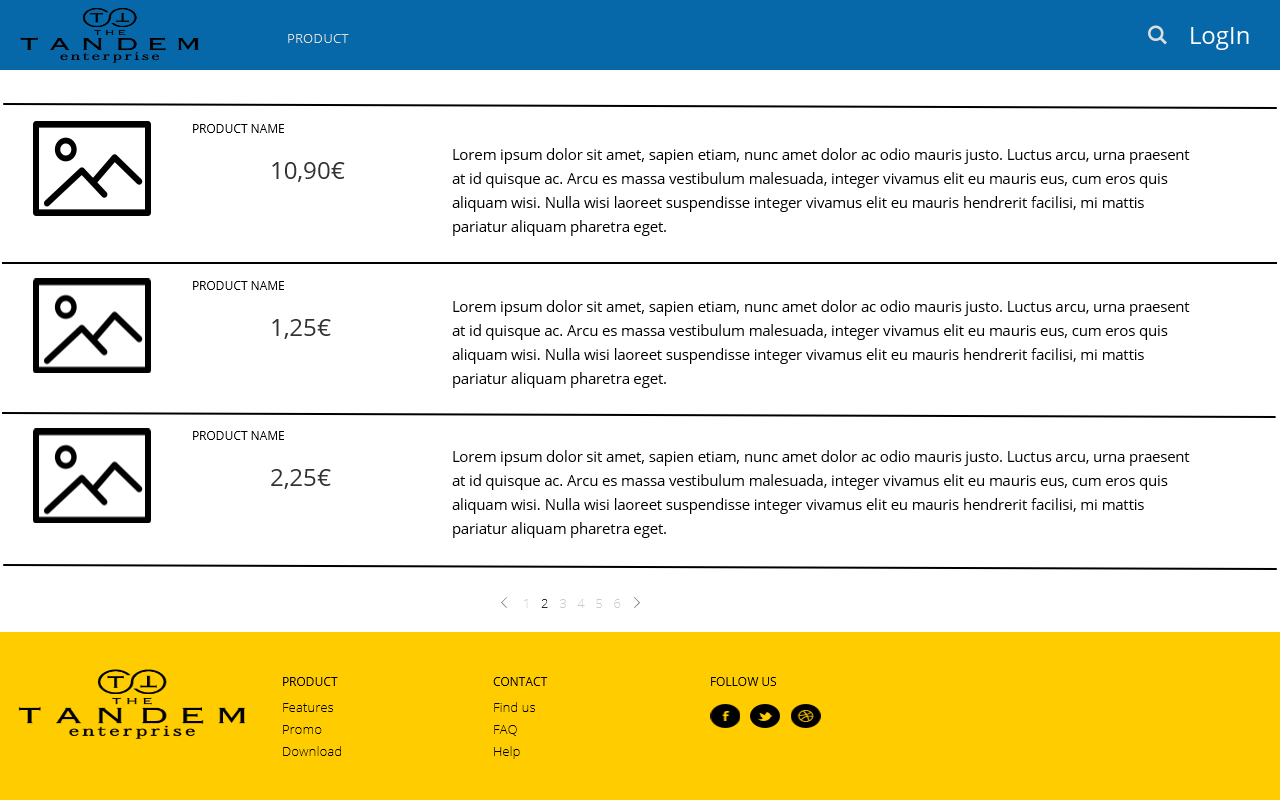
\includegraphics[scale=0.25]{mockup/Inicio.png}
    \caption{Pantalla Principal}
    \label{Fig:Inicio}
\end{figure}
\quad Esta es la pantalla principal, en cada una de las pantallas estarán presentes la barra de navegación con el logo de la empresa y las pestañas, la pestaña de login solo sera visible solo si el usuario no está registrado, si el usuario está registrado se habilitarán otras pestañas que se verán más adelante.
La pestaña de product te llevara a esta misma página y el icono de la lupa puedes buscar un producto.\\
También se mostrara el footer, donde también estarán el logo de la empresa y los contactos.\\
En esta pantalla principal se verán todos los productos disponibles con su nombre, precio y descripción. Si se clickea uno de los productos este te llevara a la propia pantalla de ese producto. 

\begin{figure}[h]
    \centering
    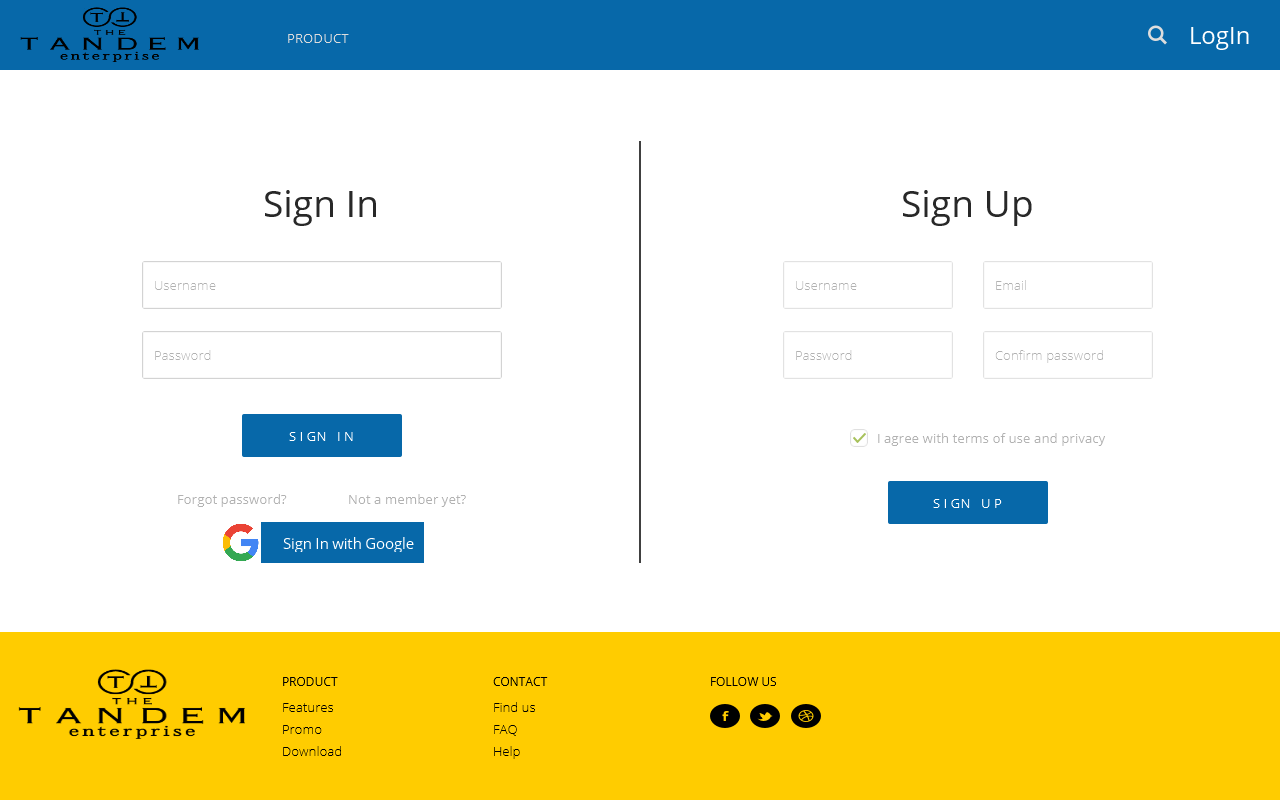
\includegraphics[scale=0.25]{mockup/Login.png}
    \caption{Iniciar sesión/Registrar usuario}
    \label{Fig:Login}
\end{figure}
\quad En esta pantalla el usuario podra iniciar sesión o registrarse.\\
Para iniciar sesión se le pedirá nombre de usuario y contraseña o en su lugar tener una cuenta con google.\\
Para registrarse solo se pedirá nombre de usuario, email, contraseña y que acepte los términos de la empresa, los datos que faltan de la tabla usuario se pedirán a la hora de realizar la compra o el usuario podra rellenarlos en su perfil como veremos más adelante.

\begin{figure}[h]
    \centering
    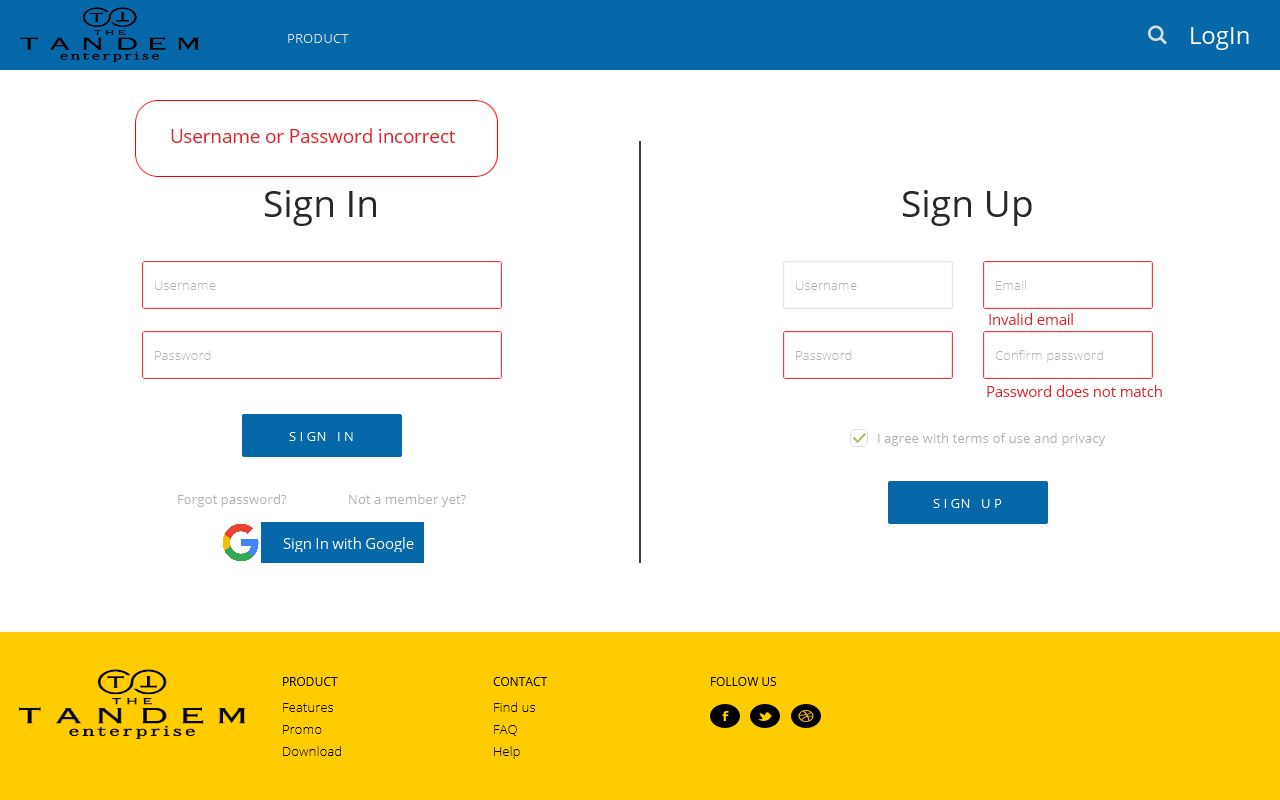
\includegraphics[scale=0.25]{mockup/Fail_login.png}
    \caption{Fallo en Iniciar sesión/Registrar usuario}
    \label{Fig:Fail_login}
\end{figure}
\quad Si el usuario comete algún error se le comunicara con estos avisos y hasta que no los corrija no podra iniciar sesión o registrarse.

\newpage

\begin{figure}[h]
    \centering
    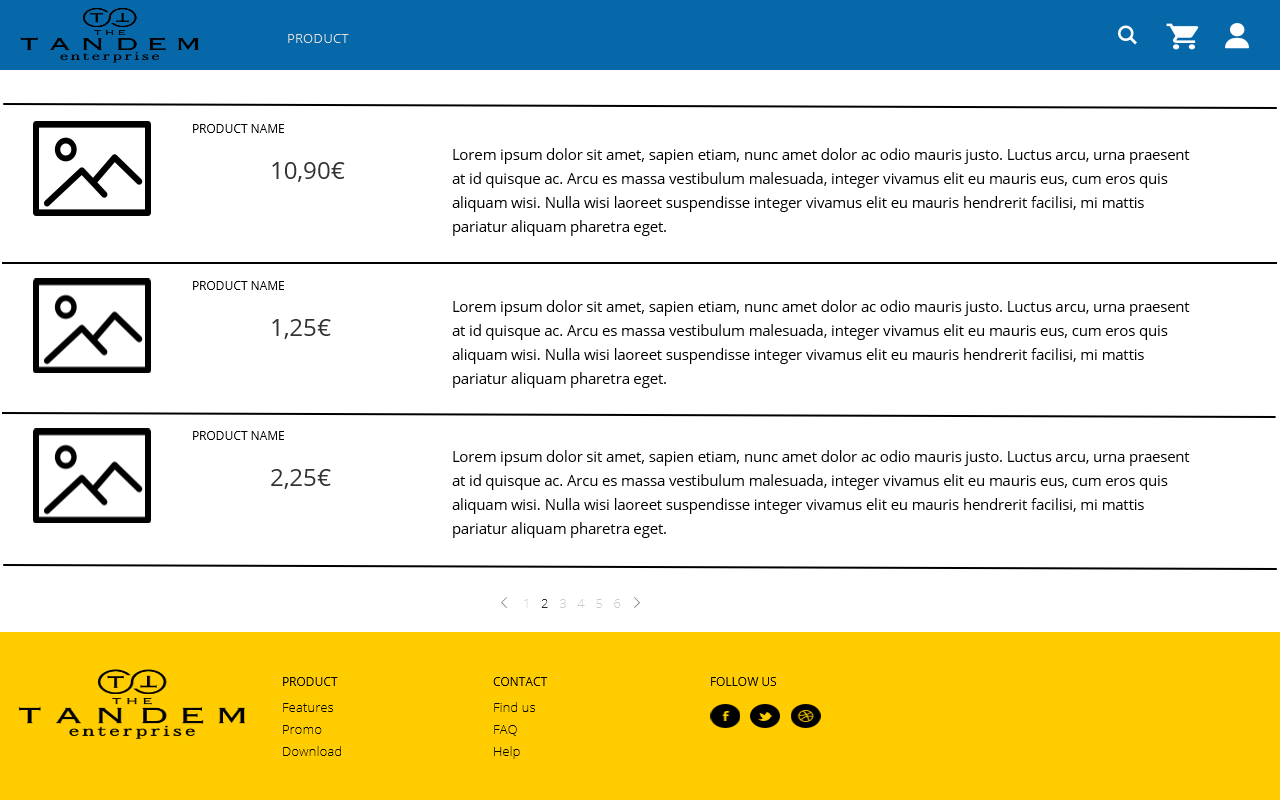
\includegraphics[scale=0.25]{mockup/Inicio_loged.png}
    \caption{Pantalla principal con usuario registrado}
    \label{Fig:Inicio_loged}
\end{figure}
\quad Cuando el usuario inicie sesión volverá a esta pantalla principal, pero ahora en vez de una pestaña login encontraremos el carrito y el perfil del usuario.
\begin{figure}[h]
    \centering
    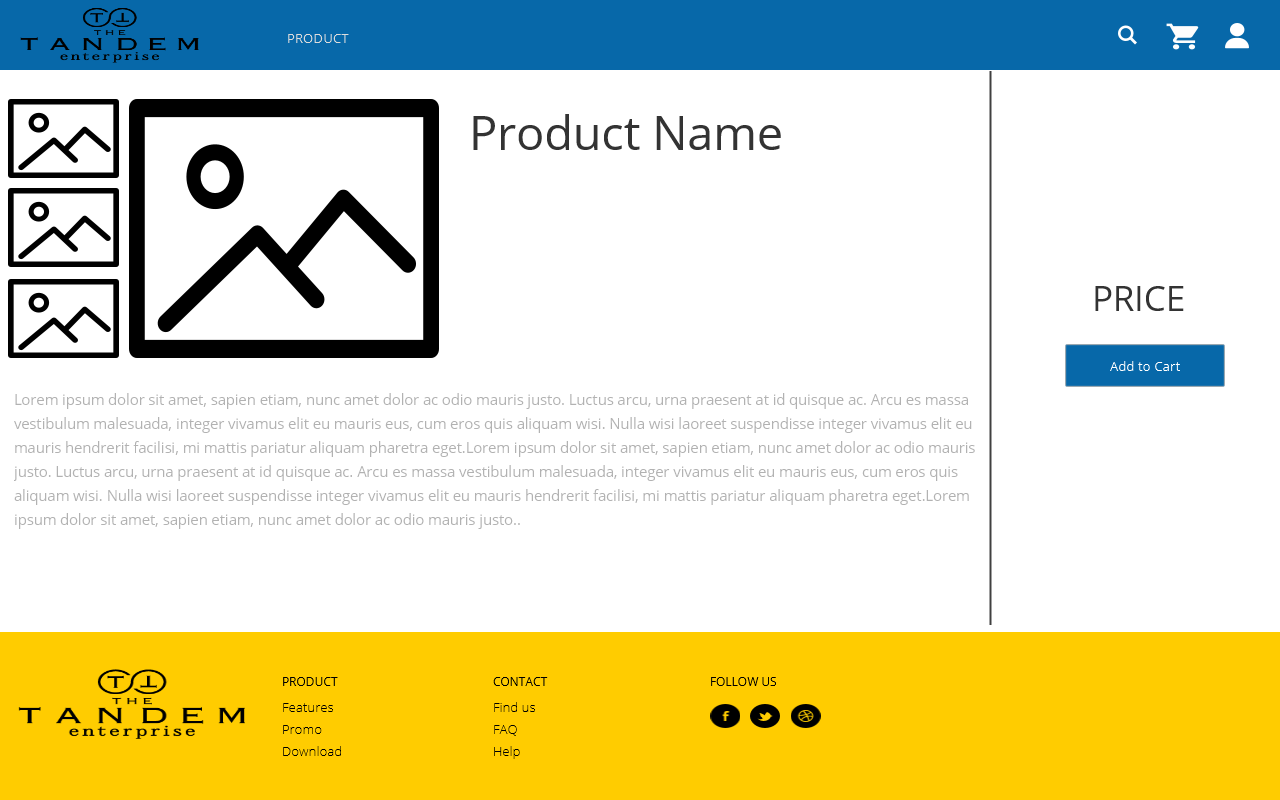
\includegraphics[scale=0.25]{mockup/product_view.png}
    \caption{Pantalla de un producto}
    \label{Fig:product_view}
\end{figure}\\
\quad Cuando el usuario quiera ver un producto le redirigirá a una pantalla de este tipo, en donde podra ver varias imágenes del producto, tendrá una descripción más amplia que en la pantalla principal y podra añadir este producto a la cesta de la compra.

\newpage
\begin{figure}[h]
    \centering
    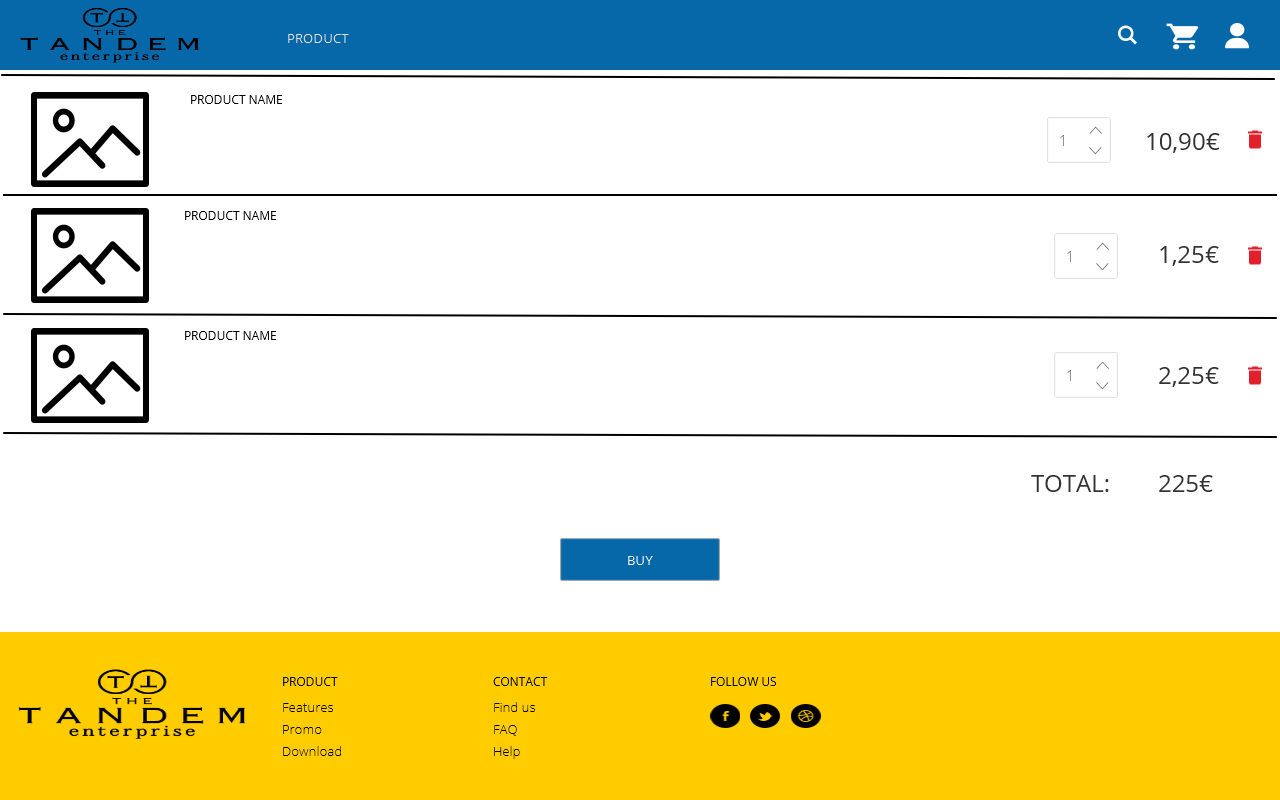
\includegraphics[scale=0.25]{mockup/cart.png}
    \caption{Pantalla del carrito de la compra}
    \label{Fig:cart}
\end{figure}
\quad Esta es la pantalla del carrito, donde el usuario podra ver los productos que ha añadido a su cesta. El usuario podra elegir la cantidad que quiere de cada producto o si quiere eliminarlo de la cesta, también podra ver el precio total de la compra y una vez ya sepa lo que quiere comprar le podra dar al botón correspondiente con esta acción (esta acción no estará implementada en este proyecto por ahora a petición de la empresa).

\begin{figure}[h]
    \centering
    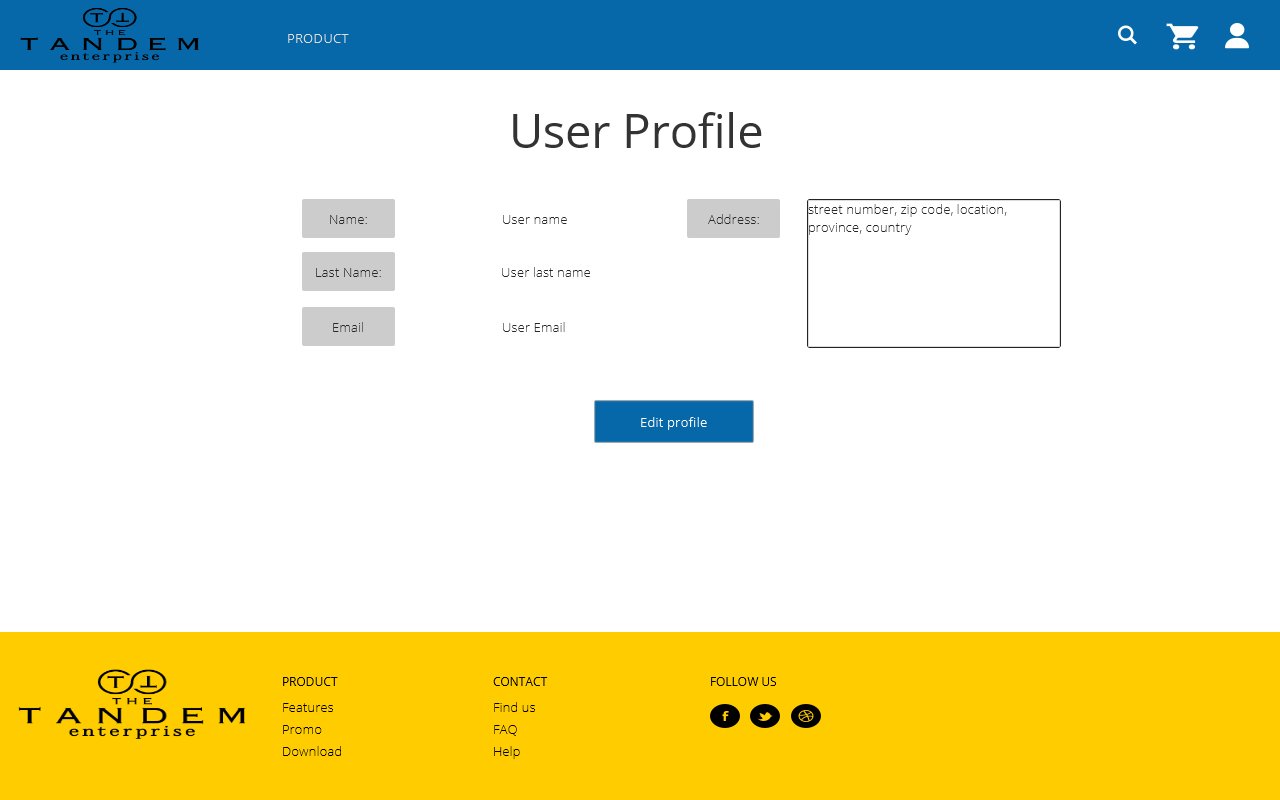
\includegraphics[scale=0.25]{mockup/Profile.png}
    \caption{Pantalla del perfil del usuario}
    \label{Fig:Profile}
\end{figure}
\quad Esta pantalla es donde el usuario podra ver sus datos y si quiere modificar algo le dará al botón de edit profile.

\newpage
\begin{figure}[h]
    \centering
    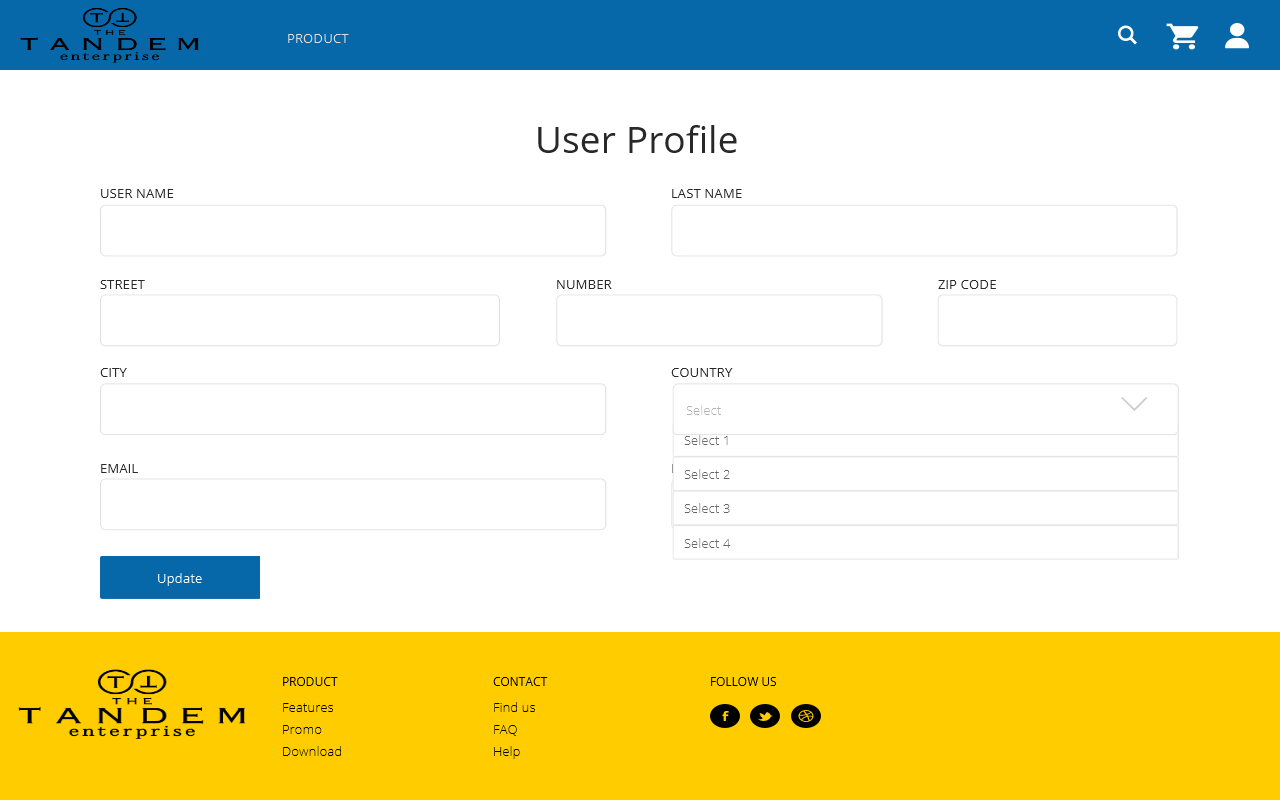
\includegraphics[scale=0.25]{mockup/Update.png}
    \caption{Pantalla para añadir o modificar datos de usuario}
    \label{Fig:Update}
\end{figure}
\quad Cuando el usuario quiera cambiar o añadir datos a su perfil sera redirigido a esta página, donde podra rellenar todos los datos relacionados con el usuario.

\begin{figure}[h]
    \centering
    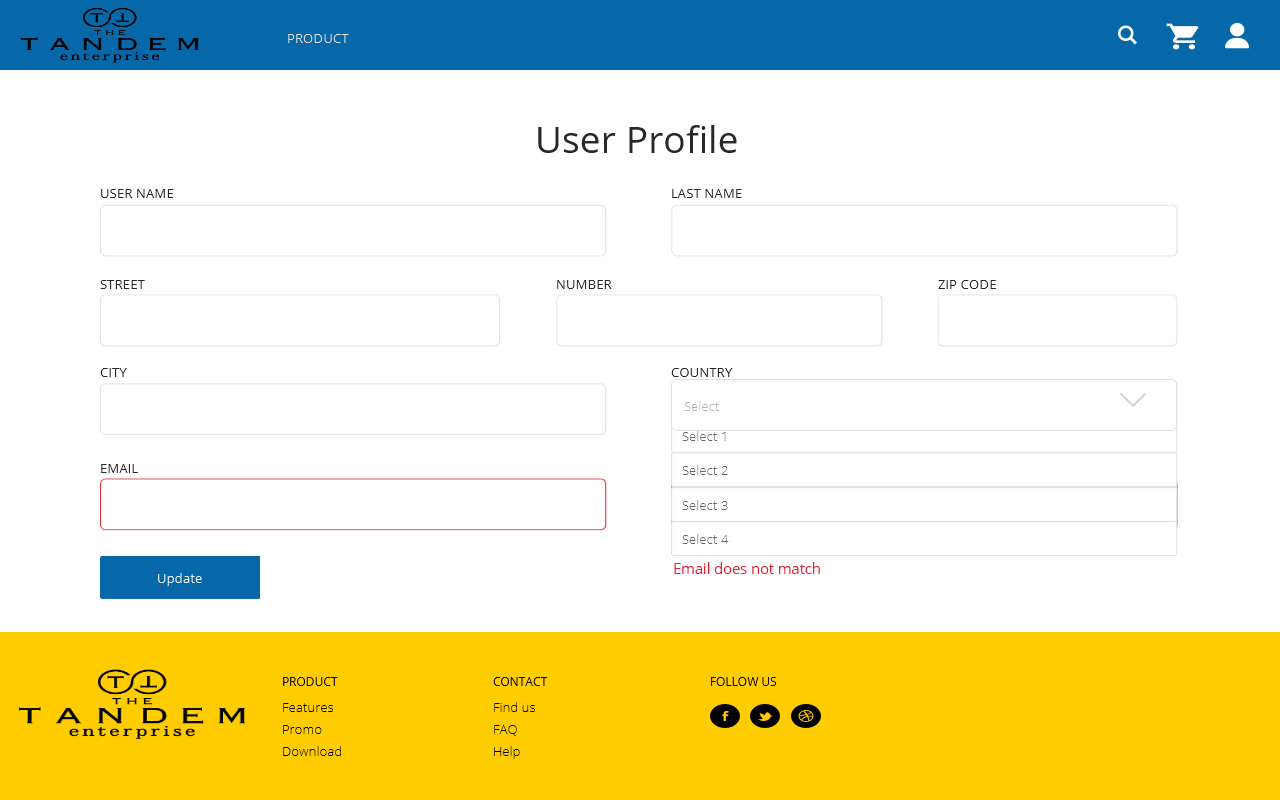
\includegraphics[scale=0.25]{mockup/Fail_update.png}
    \caption{Fallo al añadir o modificar datos de usuario}
    \label{Fig:Fail_update}
\end{figure}
\quad Si el usuario no rellena correctamente estos campos, se le avisara que campos no son correctos para que pueda corregirlos.\\

\begin{center}
    \href{https://github.com/Nestorbd/Full-Stack-Proyect/tree/master/E-commerce/Doncumentation/FullStack_Prototype}{\textbf{\textcolor{blue}{\underline{PROTOTIPO}}}}
\end{center}

\subsection{Usabilidad}
\quad Aqui vamos a ver las caracteristicas basicas de usabilidad que tiene el proyecto por ahora, fijandonos en el mockup y el prototipo:
\begin{itemize}
    \item Facil de aprender e intuitiva \\
   \phantom{ab}Estos dos puntos son complementarios, la pagina web es intuitiva ya que la estructura y funcionamiento son muy parecidos a los que se utilizan en otros sitios web dedicados al comercio como amazon y ebay.
    \item Previsión de errores\\
   \phantom{ab}Como se ve en la figura \ref{Fig:Fail_login} o en la figura \ref{Fig:Fail_update} se notificara al usuario si algún dato de los que ha introducido es erroneo.
    \item Elegante en su diseño\\
   \phantom{ab}Como se ve en el mockup y el prototipo se usara una paleta de colores basica (amarillo, blanco, azul, negro) basada en la bandera de canarias ya que se usara para vender productos canarios.
\end{itemize}
\section{Manuales}
\subsection{Instalación para desarrolladores}
\subsection{Instalación para tecnicos}
\subsection{Usuarios}
\subsection{Ayudas}
\section{Pila tecnológica}
\begin{itemize}
\item \textbf{Backend:}
\begin{itemize}
\item Node.JS
\item MySQL (BD)
\item Sequelize (ORM)
\end{itemize}
\item \textbf{Frontend:}
    \begin{itemize}
    \item Ionic-Angular
    \end{itemize}
    \item \textbf{Servicio Web:}
    \begin{itemize}
    \item RestFull
    \end{itemize}
\end{itemize}
\section{Comparación de tecnologias}
\section{Repositorios}
\begin{center}
    \href{https://github.com/Nestorbd/Full-Stack-Proyect}{\textbf{\textcolor{blue}{\underline{GitHub}}}}
\end{center}
\section{Planificación}
\section{Conclusiones, opiniones y reflexiones}
\section{Enlaces y referencias}


\end{document}